\documentclass[11pt,letterpaper]{article}
\usepackage[top=1in,bottom=1in,left=1in,right=1in]{geometry}
\usepackage[numbers]{natbib}      % http://merkel.zoneo.net/Latex/natbib.php
\usepackage{palatino}
\bibpunct{(}{)}{;}{a}{,}{,}
\usepackage{chngpage}
\usepackage{stmaryrd}
\usepackage{amssymb}
\usepackage{amsmath}
\usepackage{amsthm}
\usepackage{graphicx}
\usepackage{lscape}
\usepackage{subfigure}
\usepackage{parskip}
\usepackage[usenames,dvipsnames]{color}
\usepackage{indentfirst}
\definecolor{myblue}{rgb}{0,0.1,0.6}
\definecolor{mygreen}{rgb}{0,0.3,0.1}
\usepackage[colorlinks=true,linkcolor=black,citecolor=mygreen,urlcolor=myblue]{hyperref}
\newcommand{\bocomment}[1]{\textcolor{Bittersweet}{[#1 -BTO]}}
\newenvironment{itemizesquish}{\begin{list}{\labelitemi}{\setlength{\parskip}{0.6cm}\setlength{\itemsep}{0em}\setlength{\labelwidth}{2em}\setlength{\leftmargin}{\labelwidth}\addtolength{\leftmargin}{\labelsep}}}{\end{list}}
\newcommand{\norm}[1]{\left\lVert#1\right\rVert}
\newcommand{\ignore}[1]{}

\newcommand{\solution}[1]{{\color{Blue}[\textbf{Solution:} #1]}}
\theoremstyle{definition}
\newtheorem{question}{Question}[section]
% \newtheorem{question}{Question}
\newcommand{\rarr}{\ $\rightarrow$\ }

\bibliographystyle{plainnat}
\setlength{\parindent}{30pt}
\linespread{1}

\title{
    Speech Recognition at Baidu Research
}

\author{
	Khanh Nguyen
}

\date{June 04, 2015}

\begin{document}
\maketitle

Awni Hannun was a Stanford Ph.D. at Andrew Ng's lab and is working for him at Baidu Research. This afternoon, he gave a talk at the EE Department about works on \emph{deep learning} that have been done at Baidu to improve speech recognition. This is my attempt to write down what I have learned during this talk. 

Although speech recognition is functioning pretty well at various tasks, it is still imperfect. There are three main areas at which, according to Awni, speech recognition is struggling: (a) Noisy speech (b) Variability of the speakers (accents) (c) Natural/conversational speech. 

Here is a traditional computer vision pipeline:

\textit{Image \rarr Features \rarr Classifier}

which is very similar to the traditional speech recognition pipeline:

\textit{Speech \rarr Acoustic model \rarr Phoneme model \rarr Language model \rarr Transcription}

In this pipeline, the acoustic model recognizes the phonemes that appear in a snippet of speech. Then, the phoneme model constructs words from the phonemes. Finally, the language model decides which words should go together to form a meaningful sentence. Most of the hard works lie in designing the acoustic model. This is also where deep learning has made an impact. 

In order to train any machine learning model, one needs a loss function (or a objective function) to optimize. In the old approach for acoustic modeling, a speech snippet is chunked into "10ms" \footnote{This is a relative number.} time slices. Then each slice is matched with a phoneme in the truth text. The model defines a probability distribution of a phoneme conditional on the entire speech. The loss is the product of the probabilities over all phonemes in the truth text.  The difficulty here is to align the phonemes with the time slices. A "hack" that is often used is to give the model an initial guess of the alignment, train the model according to that alignment, then bootstrap a new (better) alignment and retrain \footnote{looks like EM to me.}.

With \emph{recurrent neural networks}, we no longer need to align phonemes. A neural network is responsible for each time slice and instead of predicting phonemes, it predicts either a single "letter" \footnote{I forget the word that he called it, which means the smallest verbal unit of a word},  a blank symbol or a stop symbol. The neural networks are then connected by \emph{bi-directional channels} across the time dimension. Here is a sketch of the model:

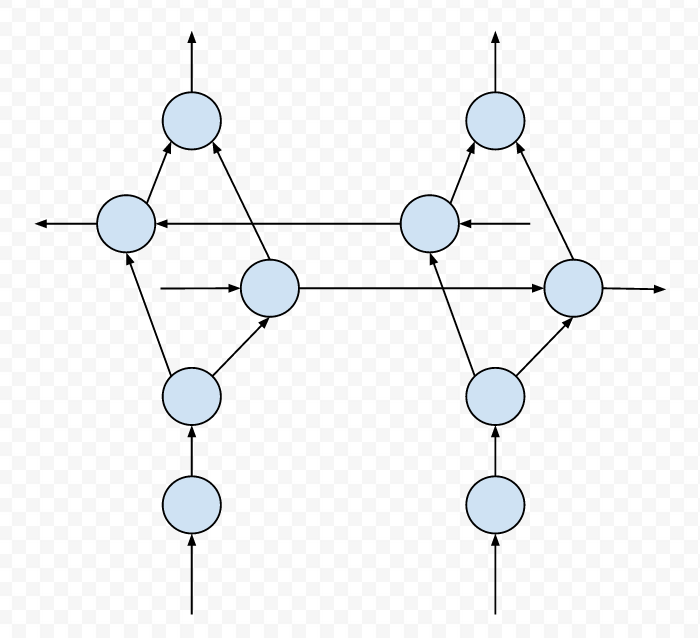
\includegraphics[width=0.5\linewidth]{baidurnn.png}

The distribution of transcribed scripts is computed by marginalize over all possible sequences. This is done using the \emph{Connectionist Temporal Classification} (or CTC) algorithm, which is a type of dynamic programming. 

An advantage of deep neural networks is that their performances are tremendously boosted with huge amounts of data. However, this also places a burden on collecting labeled data. Since the old speech recognition datasets are relatively small, Baidu researchers had to synthesize a new dataset based on the old ones. Roughly speaking, they took an original soundtrack and inserted various types and degrees of noise to create different variants of it. The final dataset consists of around $10^5$ hours of speech. 

It takes a week to train this model from scratch using mini-batch gradient descent. GPUs play an important role in speeding up this process.  The model is chopped up into parts across the time dimension and one GPU will handle each part. 

Comparing with other speech recognition systems, the Baidu systems does not gain much accuracy on clean speeches. However, it outperforms others on noisy speeches and is overall better in the combined result \footnote{The comparison is not really fair since other systems are in production so their performances may be suppressed for speed.}. Nevertheless, there is still a long way to go to be able to match with human performance on this task, which is about 2-5\% according to  Awni.

\end{document}






